\documentclass[10 pt, journal]{IEEEtran}

\usepackage{amsmath}
\usepackage{amssymb}
\usepackage[yyyymmdd]{datetime}
\usepackage{float}
\usepackage{graphicx}
\usepackage{listings}
\usepackage{subcaption}

\renewcommand{\dateseparator}{ - }
\renewcommand\IEEEkeywordsname{Keywords}

\title{Project in applied Mathematics \\
  \large Stitching used together with a virtual Pan, Tilt, Zoom camera}
\author{Adrian Roth and Filip Johannesson}

\markboth{\today}{}

\begin{document}

\maketitle
\begin{abstract}
	A conventional PTZ-camera may have the risk at looking in the ''wrong direction at the wrong time'', when surveying fast-paced scenes, such as an ongoing soccer game. An alternative to this is to simultaneously survey the entire scene, stitch the image together, and then creating the PTZ-motion in software.

	In this report we describe and implement such a system using C++ and the OpenCV 3.1.0 library. Results show that for still images, the PTZ-motion and stitching works really well. 
	When applied to snapshots from real uncalibrated cameras, results were not a good, but this might have do with poor calibration rather than the stiching and PTZ-implementation.
\end{abstract}
\begin{IEEEkeywords}
	Blending, Homography, OpenCV, PTZ, Stitching 
\end{IEEEkeywords}
\section{Introduction}
%I love image analysis and stuff. But sometimes it just sucks. Especially these times when you're supposed to write a bloody report about stuff you probably don't understand and will just bable like you do. So enjoy:
%\\\\
%Once upon a time there was a person filming another person. The movie had to be just right for it to be rewatched year after year with many laughs and tears to follow. But there was a problem. The other person, the one being filmed, was moving very fast here and there. The person filming was having trouble getting the pan, tilt and zoom of the camera correct or else something might be missed.

%Frigöra sig från linsen
%att både ha kakan och äta upp den
%best of both worlds

\IEEEPARstart{T}{racking} a plethora of moving objects, such as an ongoing soccer game, with a mechanical Pan, Tilt, Zoom (from here on PTZ) can be a somewhat daunting task.
With things happening all over the surveyed scene and the sometimes significant response time of actuators in the PTZ-camera, there is a real possibillity that the camera is pointed in the ''wrong direction at the wrong time'', see fig. \ref{fig:problem}.

\begin{figure}[H]
	\centering
	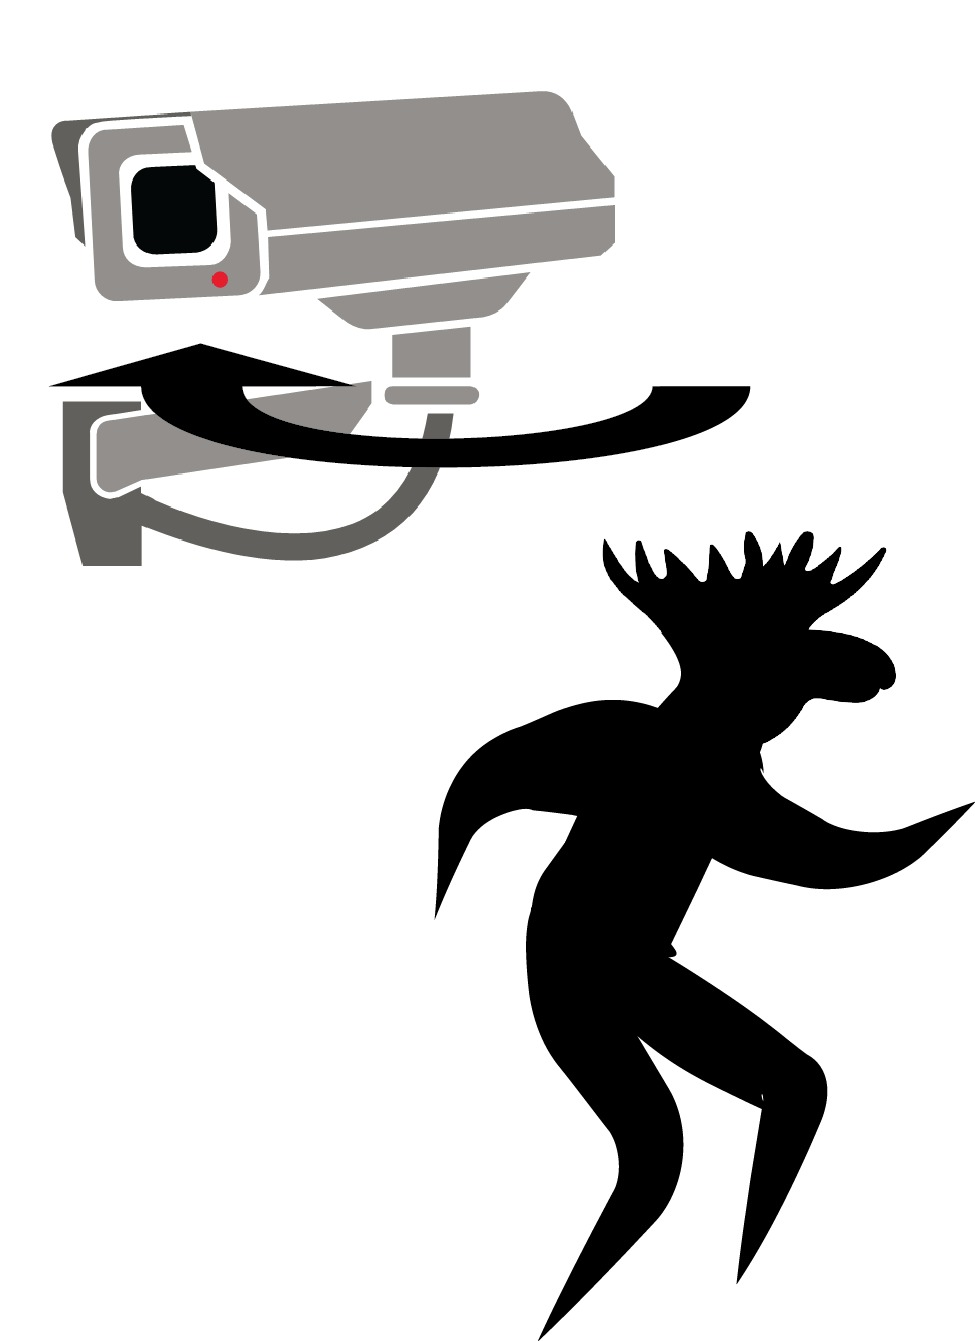
\includegraphics[width=0.5 \columnwidth]{../results/images/PTZ_problem.jpg}
	\caption{A panable camera looking in the wrong direction, therby not noticing a moose sneaking by.}
	\label{fig:problem}
\end{figure}

In this project we investigate another method, where multiple stationary cameras are used to cover the entire scene under surveillance, and then produce the PTZ-motion in software by panoramic stitching and virtual cameras.
A conceptual depiction of the system can be seen in fig. \ref{fig:comp}.

\begin{figure}[H]
	\centering
	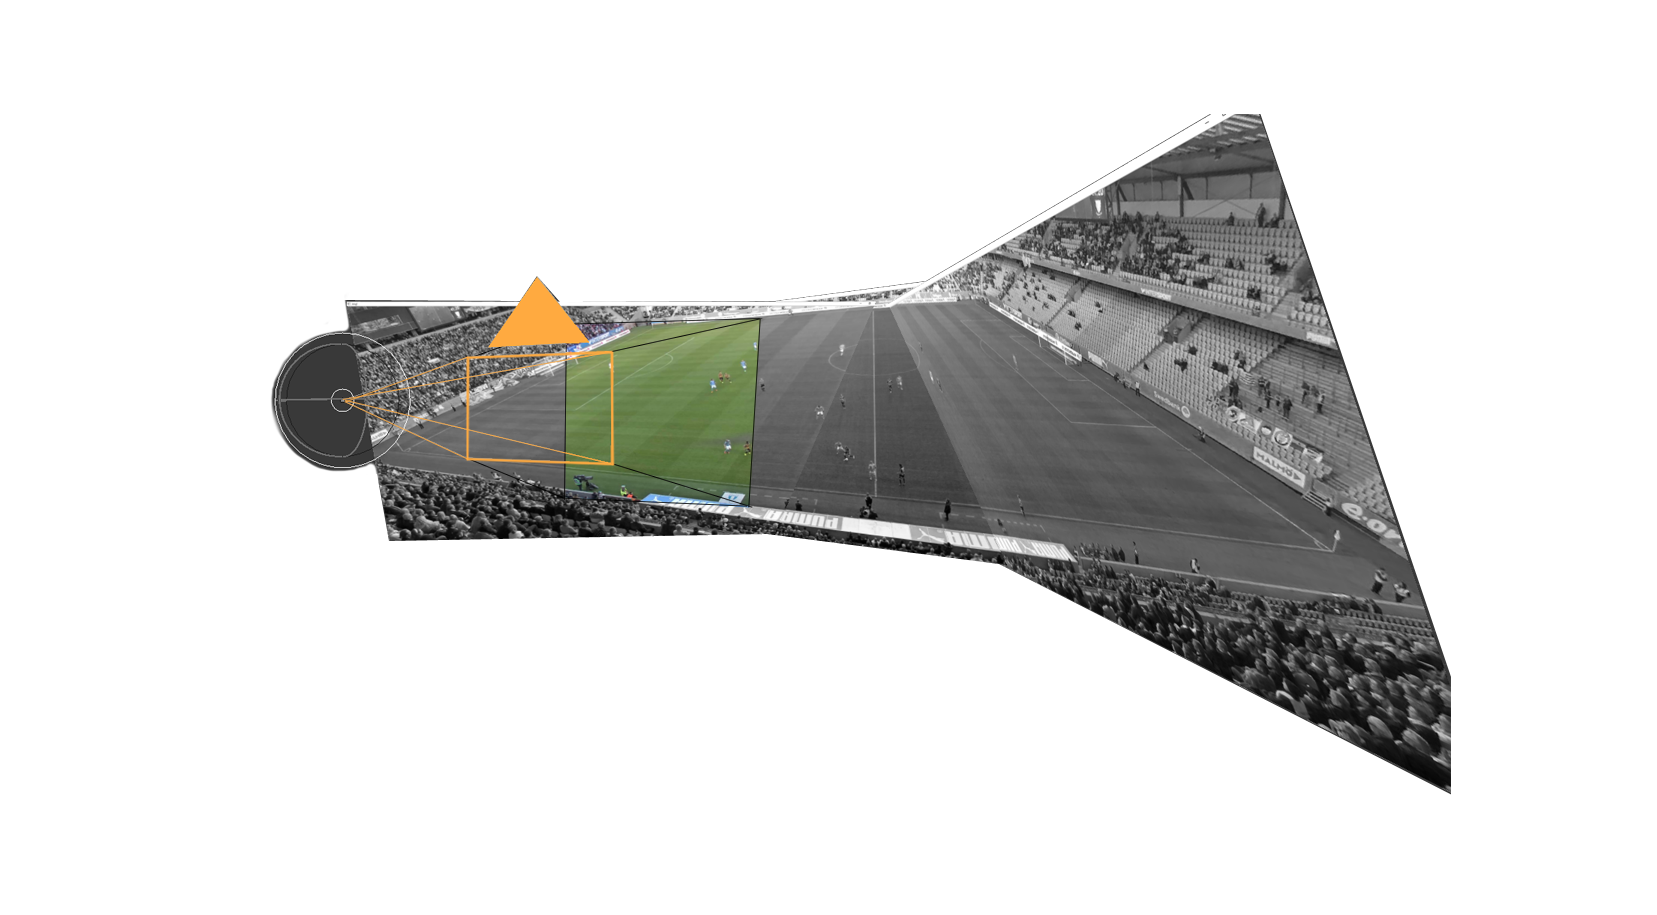
\includegraphics[width=0.7\columnwidth]{../results/images/PTZ_comp.png}
	\caption{A concept drawing of a virtual PTZ-camera. The input images are transformed and stitched together to form a ''curved'', stitched image of the entire scene. The virtual camera can then be seen as putting a new camera in front of this ''curved image'', where the pan and tilts are essentially rotations of the virtual camera. Zooming can be thought like magnification or reduction of the stitched image.}
	\label{fig:comp}
\end{figure}


\section{Theory}


\section{Method}

The program can be thought of a modifed image stitching pipline, with stages:
\begin{enumerate}
	\item Find Surf features in input images
	\item Estimate homographies between input images
	\item Create the virtual camera
	\item Pan/Tilt and Zoom with virtual camera to create PTZ transformation matrix
	\item Create a composite transformation matrix.
	\item Apply transformations on input images.
	\item Blend transformed images.
\end{enumerate}

In this particular implementation three images depicting a soccer game were used, as can be seen in fig.\ref{fig:input}.
From the implementation the most important functionality from OpenCV can be found in appendix \ref{appendix:opencv}.

\begin{figure*}[t]
	\centering
	\begin{subfigure}[t]{0.3\textwidth}
		\centering
		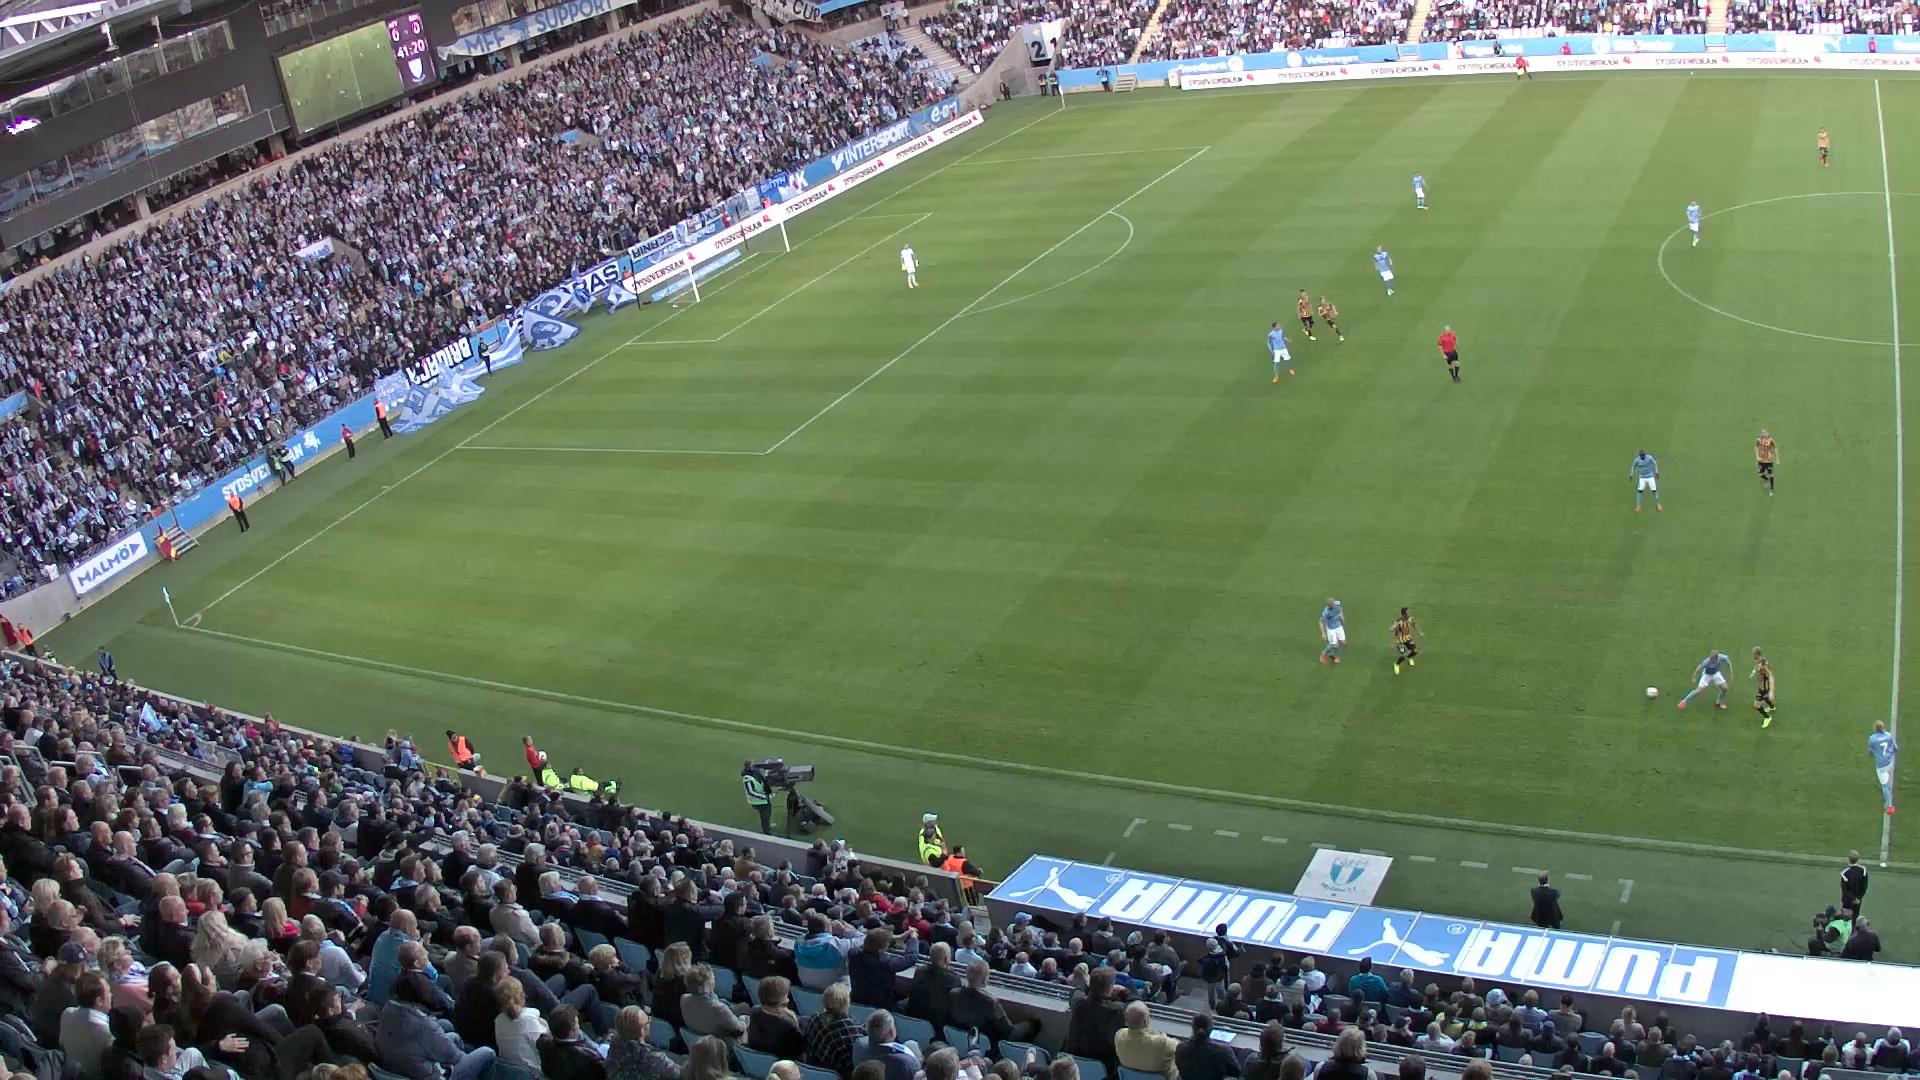
\includegraphics[width=\textwidth]{../data/20150521_194353_C1D8.jpg}
		\caption{1}
	\end{subfigure}
	\begin{subfigure}[t]{0.3\textwidth}
		\centering
		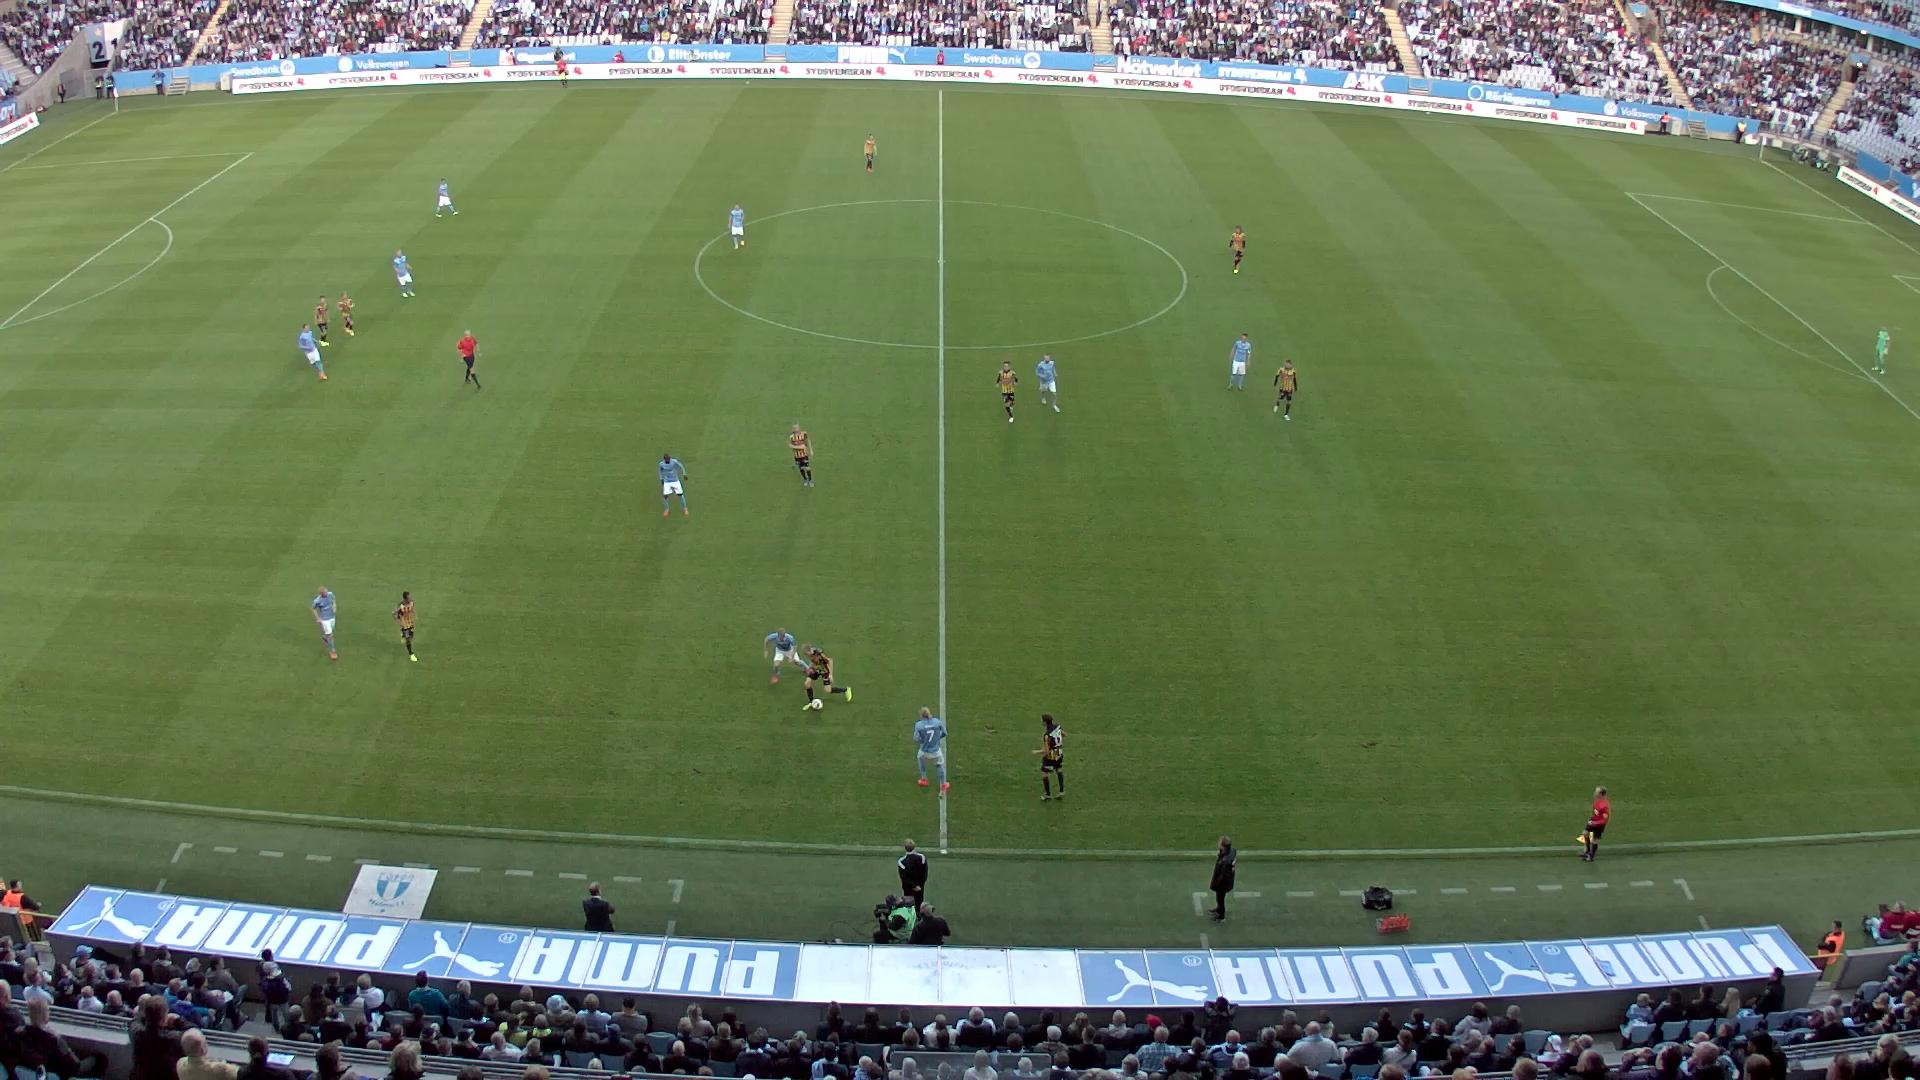
\includegraphics[width=\textwidth]{../data/20150521_194353_FD1E.jpg}
		\caption{2}
	\end{subfigure}
		\begin{subfigure}[t]{0.3\textwidth}
		\centering
		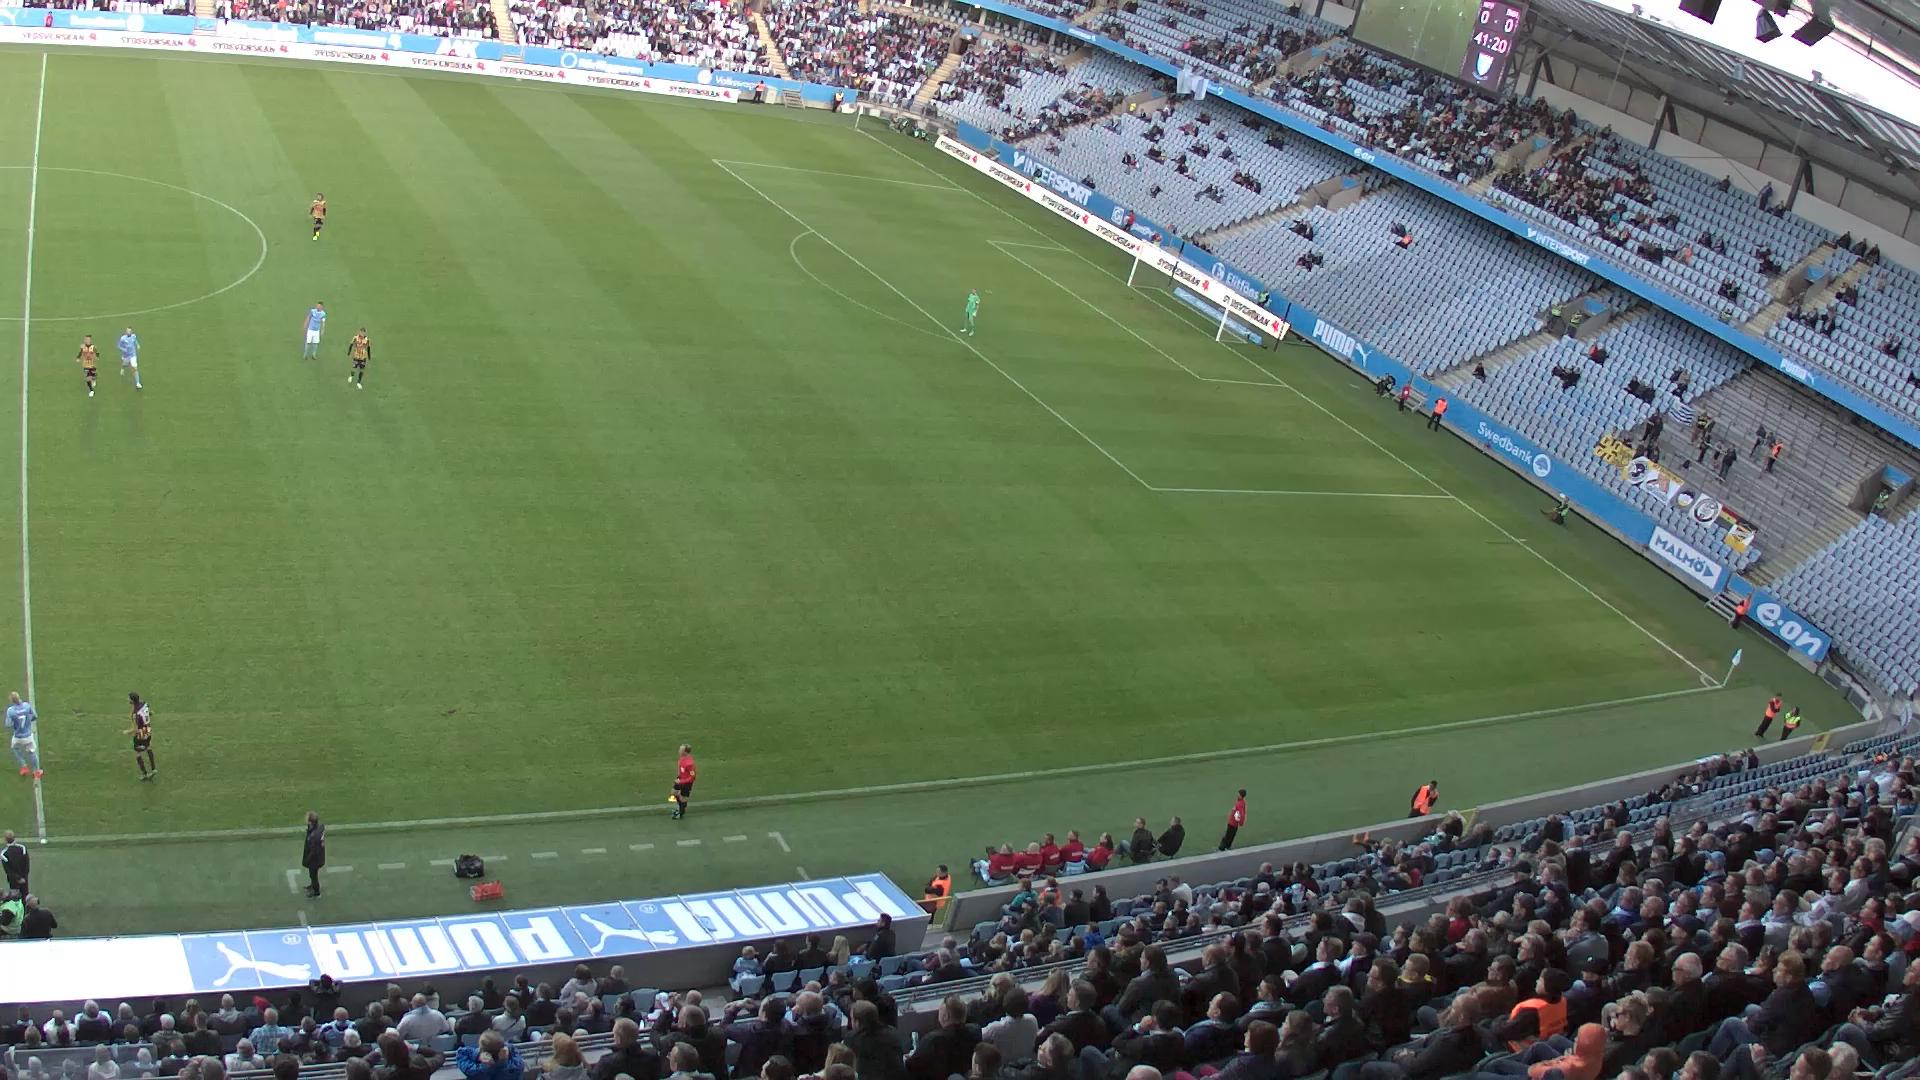
\includegraphics[width=\textwidth]{../data/20150521_194353_49E3.jpg}
		\caption{3}
	\end{subfigure}
	\caption{input images}
	\label{fig:input}
\end{figure*}

\subsection{Stitching}
This text only refers to stitching of two images, the same concept can be expanded for multiple images.

The stitching can be divided into two parts.
The first one is to find a relation, homography, between two images.
In other words where an image {\it fits} in the other image.
The other part is to combine or blend the images to make the transition between them as smooth as possible.

To find a relation between two images, mutual points have to be found.
This is done using a point detector which should find interest points in both images.
Then the points need a value for the possibility of matching points that are similar.
Here a feature descriptor is needed.
In this project a method called SURF has been used.
It includes both a detector and descriptor.
After SURFing the images the descriptors of the points are matched.
This matching is very likely to contain outliers, however, the RANSAC method can be used to avoid influence of the outliers when calculating the homography between the images.

The blending of the two images consists of three steps.
First the previously calculated homography is used to get the images in the same perspective.
Here there is an overlap between the images.
This overlap is weighted with a value $w_1$ for the left image and $w_2 = 1 - w_1$ for the right one.
In this project $w_1$ has been calculating using either a linear (equation \ref{eq:method:stitching:linear}) or sigmoid (equation \ref{eq:method:stitching:sigmoid}) function.
\begin{equation} \label{eq:method:stitching:linear}
  w_1 = -a x + b
\end{equation}
\begin{equation} \label{eq:method:stitching:sigmoid}
  w_1 = \frac{e^{-0.1(x - x_d)}}{1 + e^{-0.1(x - x_d)}}
\end{equation}
Here $a$, $b$ and $x_d$ are adapted to fit the overlap of the images.
With the start and end of the overlap in the x-direction a and b are set so that $w_1 = 1$ on the left end and $w_1 = 0$ on the other.
$x_d$ is just set to be the in the middle of the overlap in the x-direction.
At last the weighted images are stitched together.


\subsection{Virtual PTZ camera}
Using the decomposition in (\ref{eq:homodecomp}) we can transform the problem into three rotations, where we only really need to use two of them, the panning rotation around the camera Y-axis and rotation around the camera X-axis after the panning has been applied.
The rotational matrices are implemented as follows in (\ref{eq:pan}) and (\ref{eq:tilt})
	\begin{align}		
		R_{pan}&=\begin{pmatrix} 
			\cos(\theta_y) & 0 & -\sin(\theta_y) \\
			0 & 1 & 0 \\
			\sin(\theta_y) & 0 & \cos(\theta_y)
		\end{pmatrix} \label{eq:pan} \\
		R_{tilt} &=\begin{pmatrix}
			1 & 0 & 0 \\
			0 & \cos(\theta_x) & -\sin(\theta_x) \\
			0 & \sin(\theta_x) & \cos(\theta_x)
		\end{pmatrix} \label{eq:tilt}
	\end{align}
	For the particular input images in fig. \ref{fig:input}, the cameras were slighty tilted , with an estimated initial tilt angle of $\approx 0.47$ radians.\footnote{The exact estimated angle was 0.47179832679 radians.}
	This means that if we want our panning axis to coincide with the panning axis of the input images, we first need to apply a tilting of $-0.47$ radians, and then apply our panning matrix, (\ref{eq:pan}) and then our tilting matrix. 
	The ''initial tilt correction'' can be written in matrix form as (\ref{eq:tiltinit}).
	\begin{multline}
		R_{tiltCorr}=\begin{pmatrix}
			1 & 0 & 0 \\
			0 & \cos(-\theta_{tiltinit}) & -\sin(-\theta_{tiltinit}) \\
			0 & \sin(-\theta_{tiltinit}) & \cos(-\theta_{tiltinit})
		\end{pmatrix} = \\
		=\begin{pmatrix}
			1 & 0 & 0 \\
			0 & \cos(\theta_{tiltinit}) & \sin(\theta_{tiltinit}) \\
			0 & -\sin(\theta_{tiltinit}) & \cos(\theta_{tiltinit})
		\end{pmatrix}
		\label{eq:tiltinit}
	\end{multline}
	where $\theta_{tiltinit} \approx 0.47$ radians.

	The zoom is implemented as stated in (\ref{eq:zoom}).
	The matrices are finally multiplied together to a single composite matrix, $H_{perspective}$, see (\ref{eq:PTZcomp})

	\begin{equation}
		H_{perspective}=KZR_{tilt}R_{pan}R_{tiltCorr}K^{-1}
		\label{eq:PTZcomp}
	\end{equation}
	where K are the camera calibration matrices.
	As stated in the theory section, the homographies applied on the images are variants of a composite matrix defined as in (\ref{eq:comp}).

	\begin{equation}
		H_{composite}=H_{perspective}H_{stitching}
		\label{eq:comp}
	\end{equation}
	Where $H_{stitching}$ is the homography produced by the stitching algorithm, invidiual for each image. Note that the stitching transform is applied prior to the perspective transforms. % is it not the other way around



\section{Results}

\subsection{Stitching}
The stitching was performed with two different blending functions.
The result of stitching image one and two with a linear transition is shown in fig. \ref{fig:results:stitching:linear} and the corresponding one using a sigmoid function is shown in fig. \ref{fig:results:stitching:sigmoid}.
The resulting stitched scene using the provided input images, fig. \ref{fig:input} can be seen in fig. \ref{fig:res_stitch}.
A stitching was also performed when using two cameras in a home made set-up, it is found in fig. \ref{fig:results:stitching:homemade}.

\begin{figure}[H]
  \centering
  \includegraphics[width = 0.9\columnwidth]{../results/stitch_linear.jpg}
  \caption{Stitching done using a linear transition.}
  \label{fig:results:stitching:linear}
\end{figure}

\begin{figure}[H]
  \centering
  \includegraphics[width = 0.9\columnwidth]{../results/stitch_sigmoid.jpg}
  \caption{Stitching done using a sigmoid transition.}
  \label{fig:results:stitching:sigmoid}
\end{figure}

\begin{figure*}
	\centering
	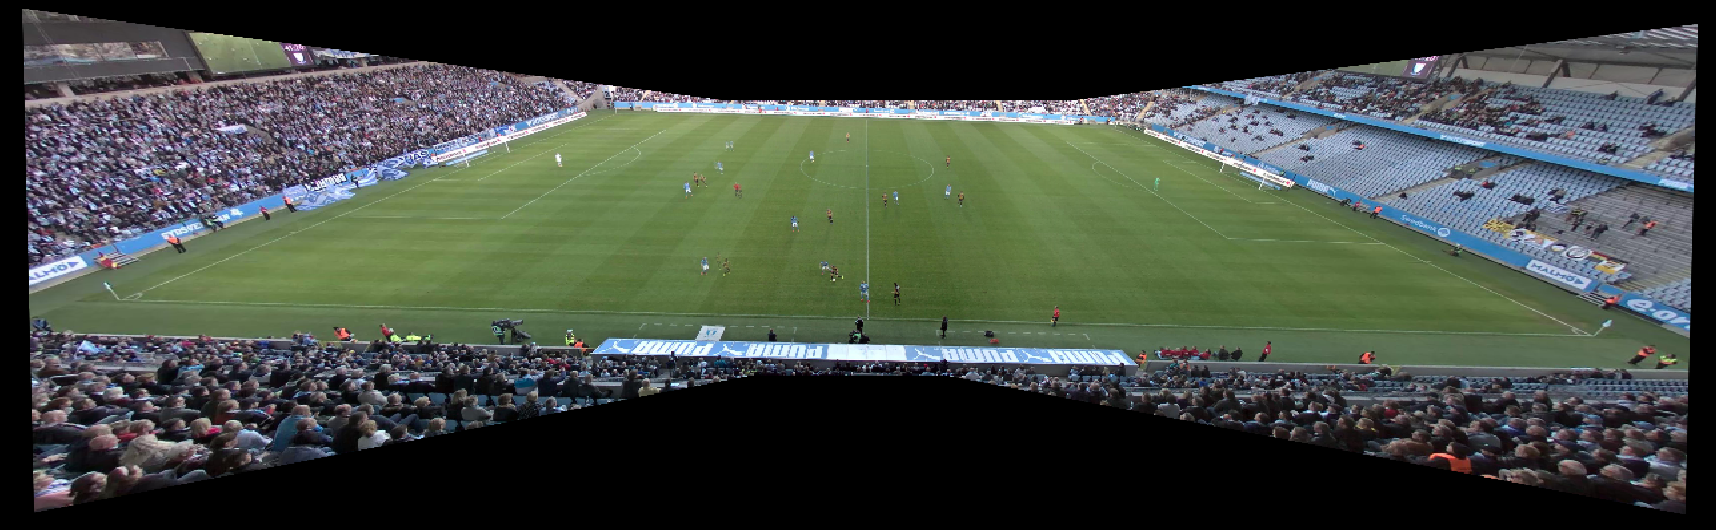
\includegraphics[width=0.8\textwidth]{../results/images/res_stitch.PNG}
	\caption{All three input images stitched together}
	\label{fig:res_stitch}
\end{figure*}

\begin{figure*}
	\centering
	\begin{subfigure}[t]{0.3\textwidth}
		\centering
		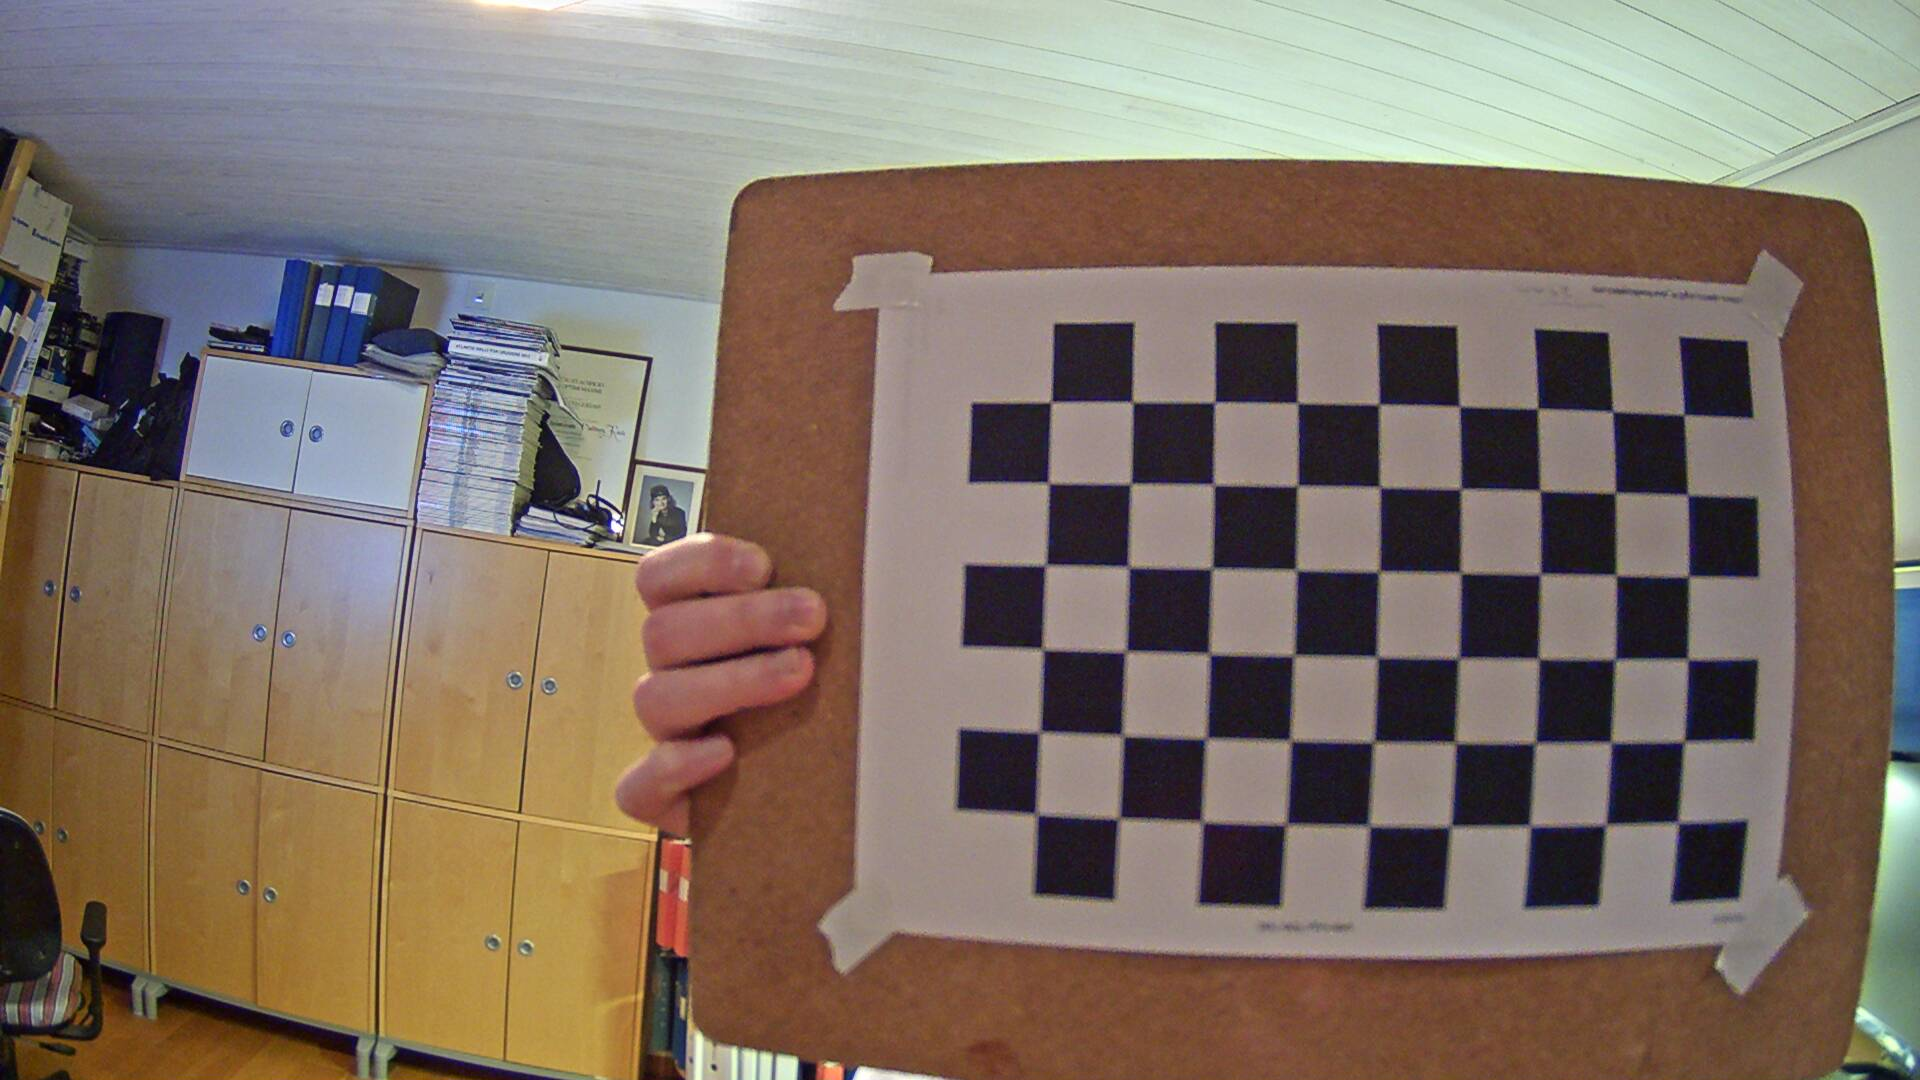
\includegraphics[width=\textwidth]{../results/camera_1.jpg}
		\caption{input 1}
	\end{subfigure}
	\begin{subfigure}[t]{0.3\textwidth}
		\centering
		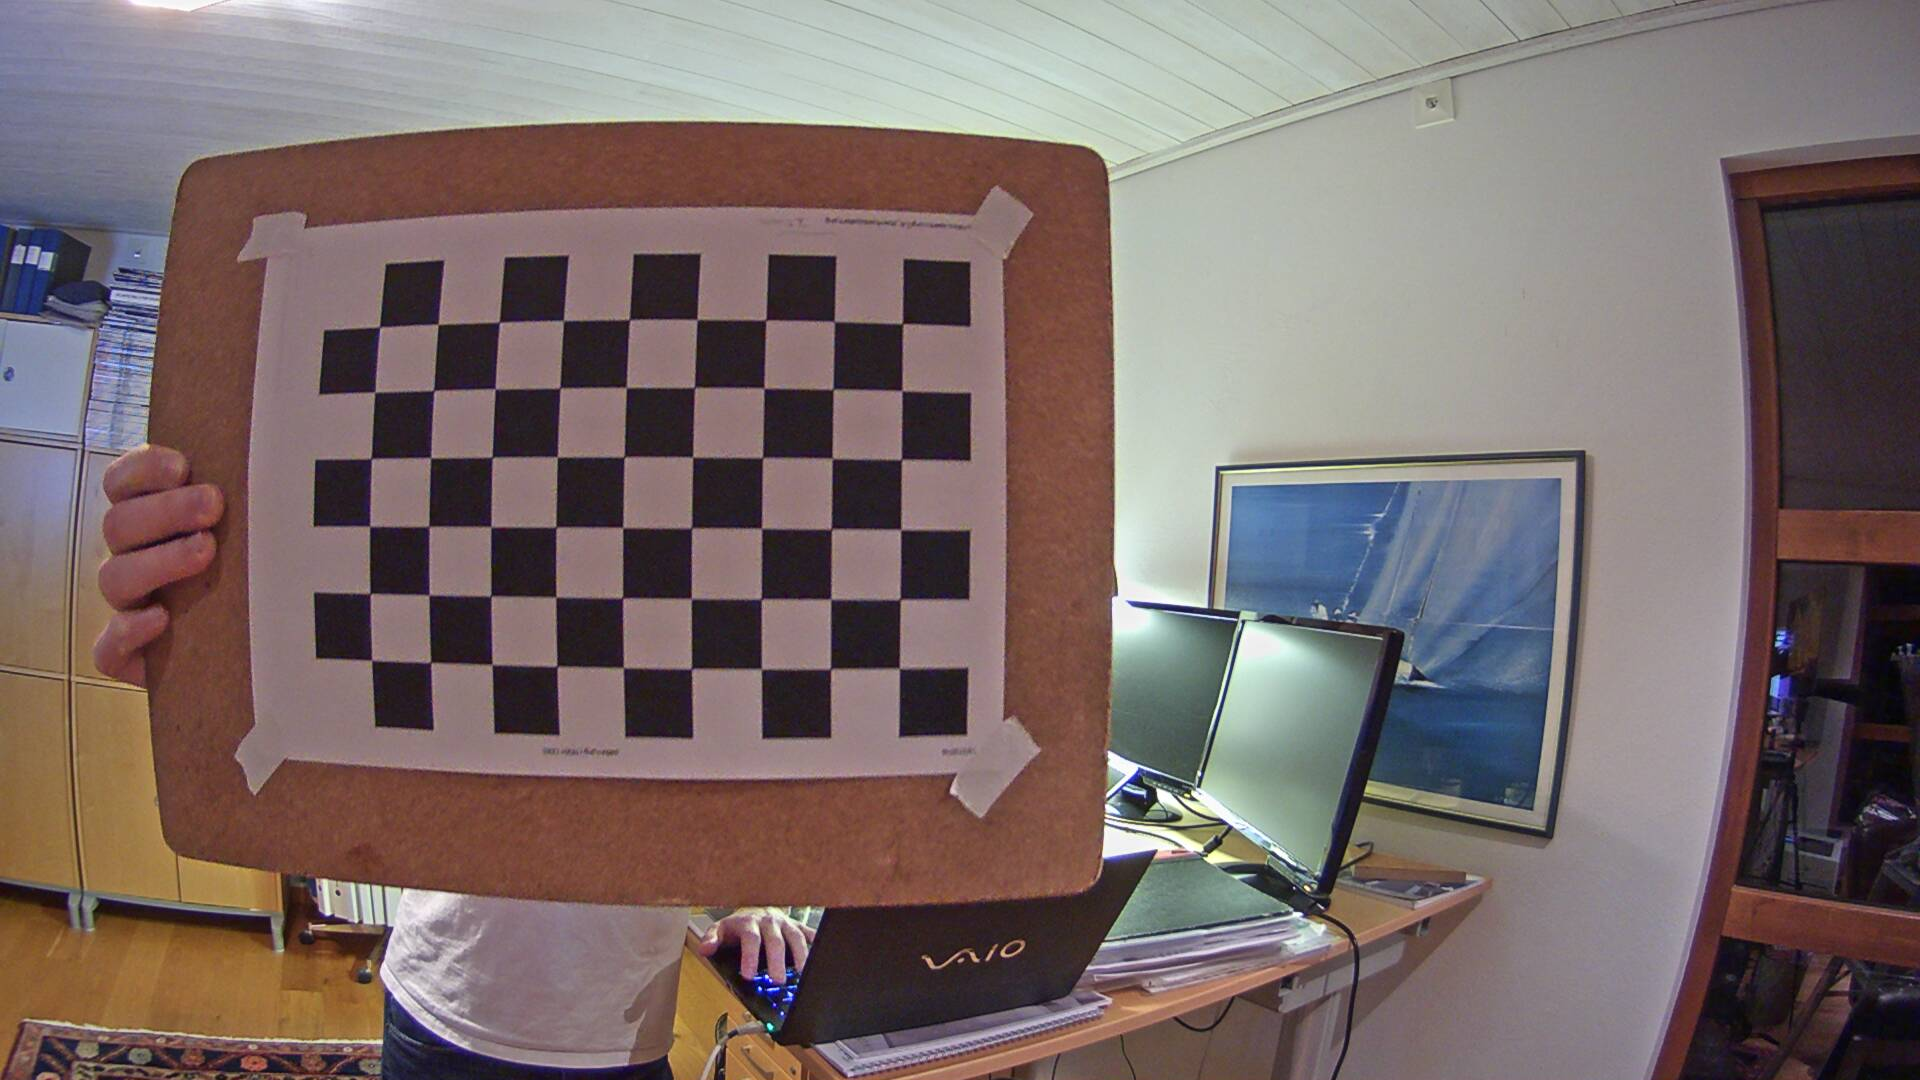
\includegraphics[width=\textwidth]{../results/camera_2.jpg}
		\caption{input 2}
	\end{subfigure}
		\begin{subfigure}[t]{0.3\textwidth}
		\centering
                \includegraphics[width = \textwidth]{../results/home_made_stitch.jpg}
		\caption{output}
	\end{subfigure}
        \caption{Stitching done with home made set-up.}
	\label{fig:results:stitching:homemade}
\end{figure*}


\subsection{Virtual PTZ camera}
Initially, some simple transformations were carried out in MATLAB using a symmetrical set of normalized homogeneous points, i.e. four points with coordinates (-1,-1,1), (1,-1,1), (1,1,1) and (-1,1,1) in $\mathbb{P}^2$.

Secondary trials were made with a point set with origo in a corner point, similar to the coordinate system in an image.
Here {\it calibration} matrices were needed in order to move the image origo to the center of the image and scale it.

Advancements into real-images were then straight forward as the synthezised calibration matrices were replaced with the real calibration matrices.
The resulting PTZ movement can be seen in fig. \ref{fig:ptz_res}.

\begin{figure}[H]
	\centering
	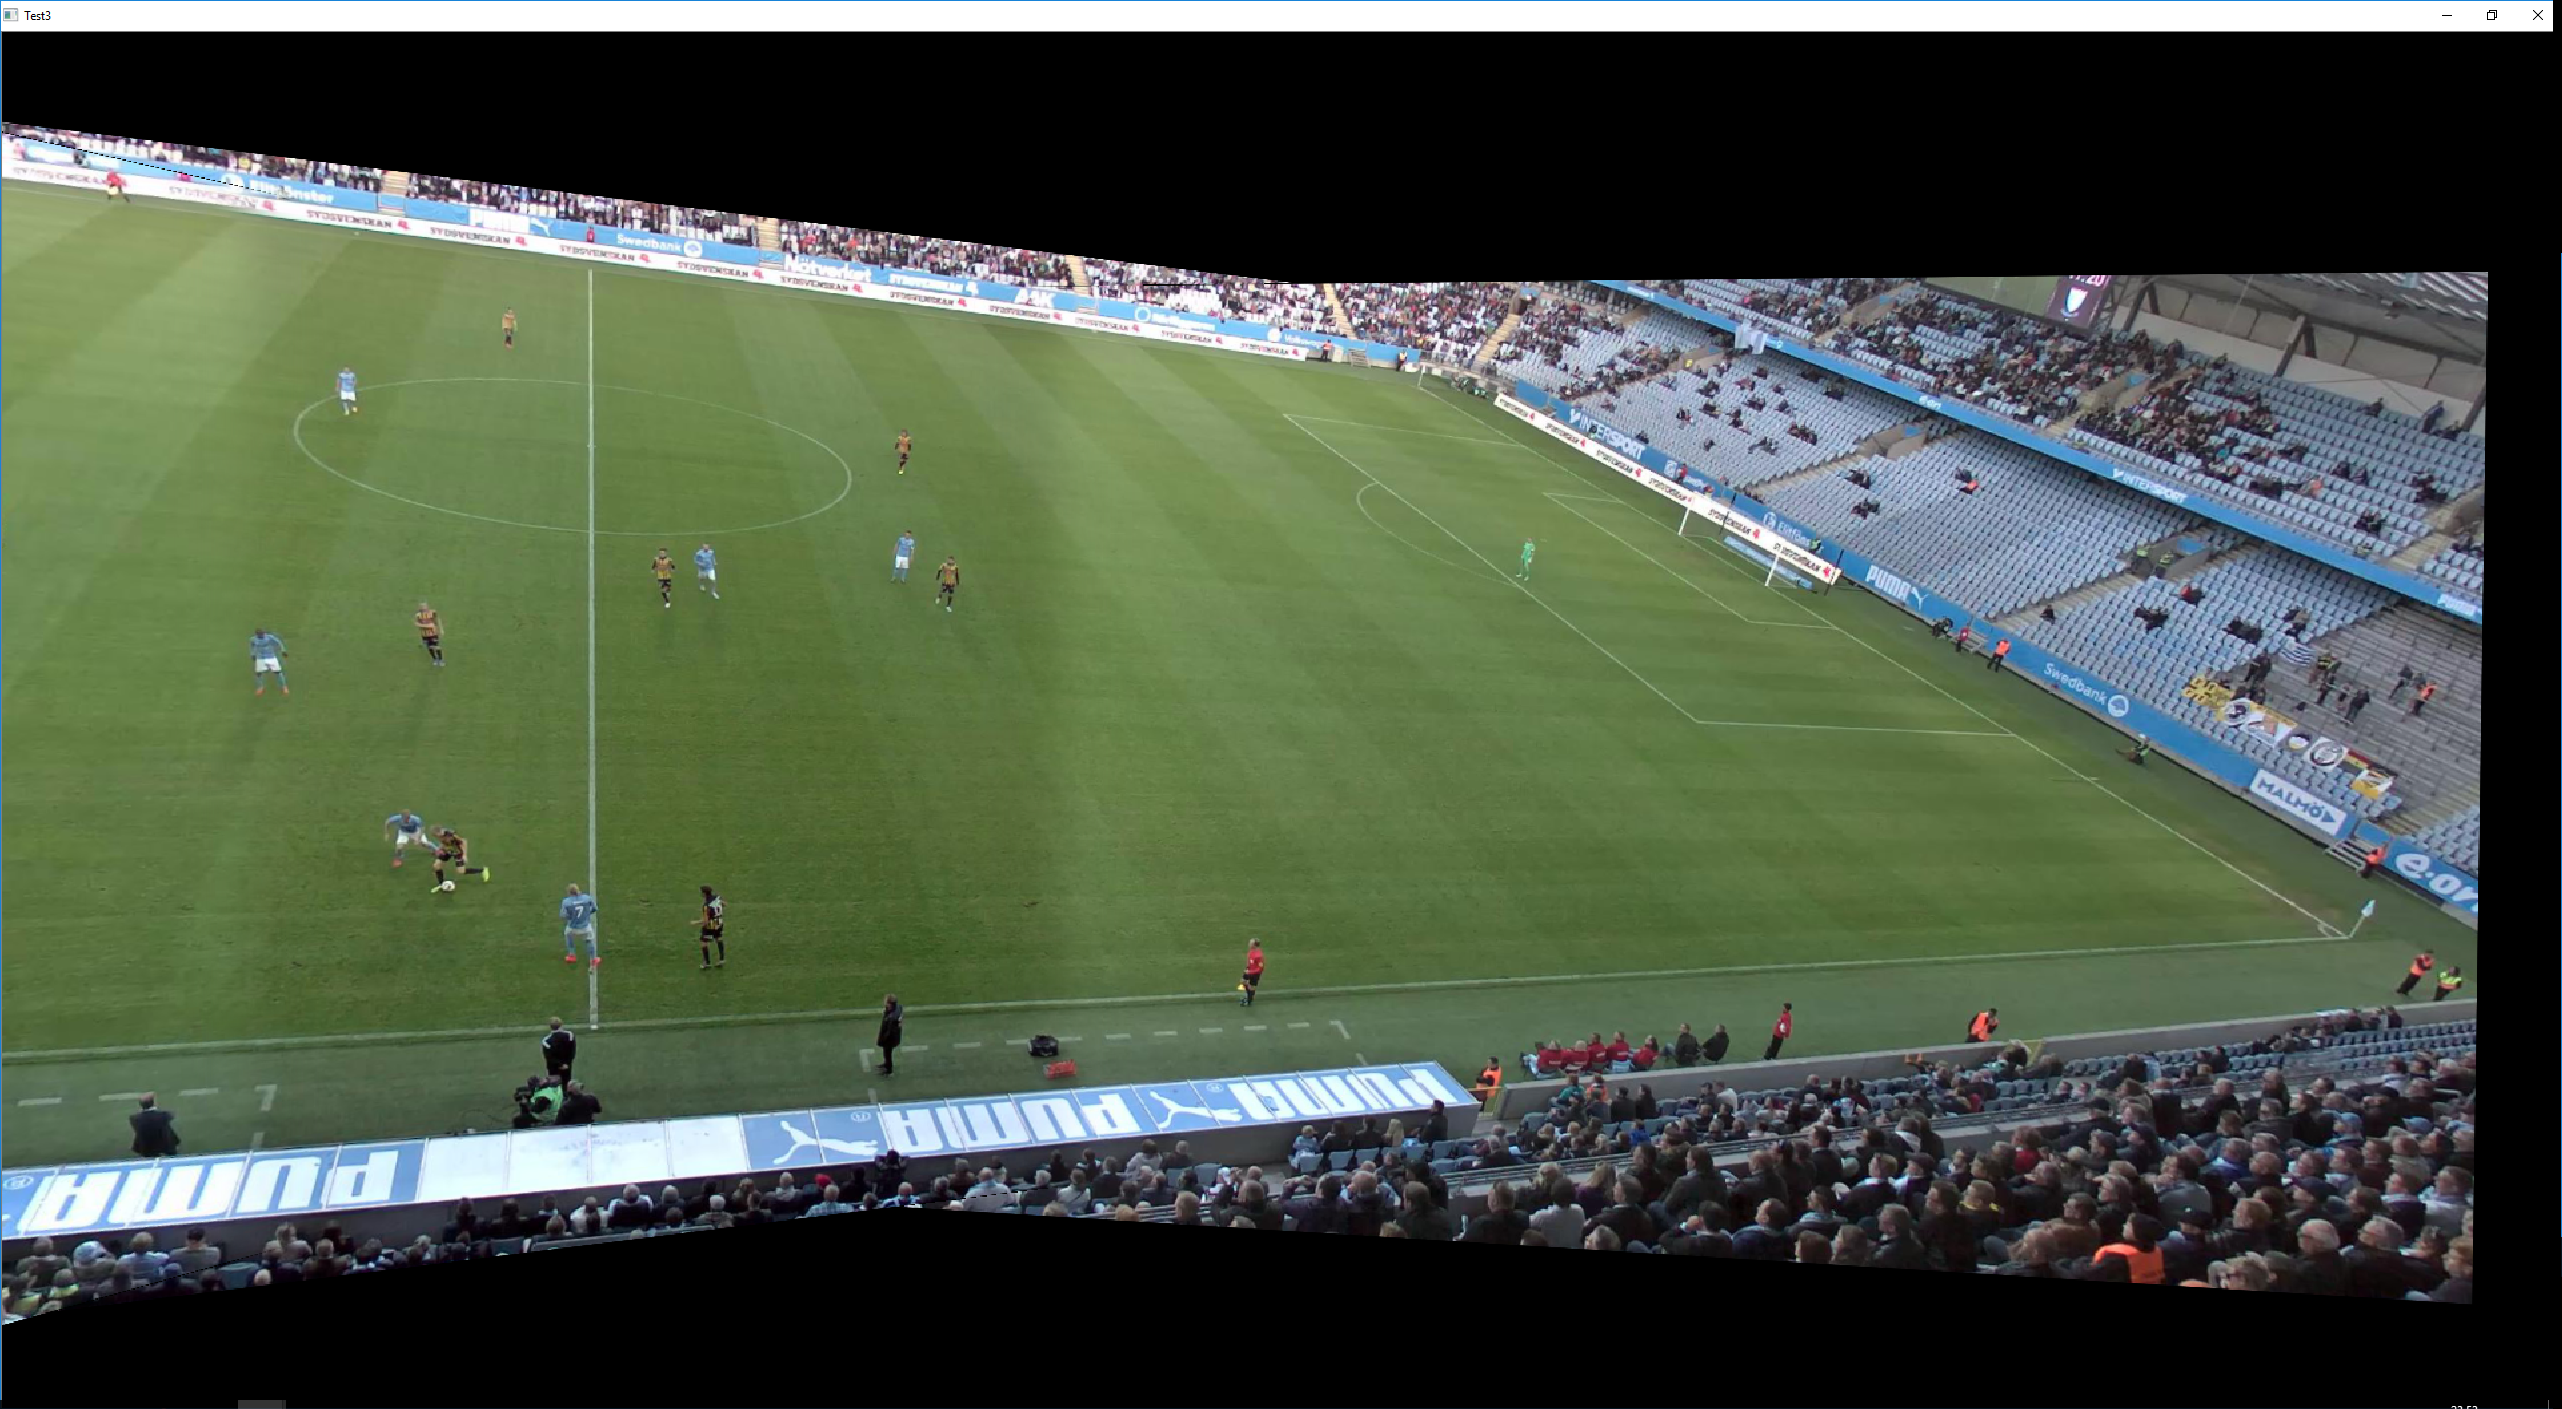
\includegraphics[width=0.8\columnwidth]{../results/images/PTZ_res.PNG}
	\caption{An example of the resulting image where the virtual camera has been panned, tilted and zoomed.}
	\label{fig:ptz_res}
\end{figure}



\section{Discussion}
For the stitching there two different blending functions were used as seen in fig. \ref{fig:results:stitching:linear} and \ref{fig:results:stitching:sigmoid}. The blending first of all reveals that the images are not taken at the same time. This means that the scene has changed betwen the images. With this in mind the sigmoid function gives a better result, a smoother transition in the stitching. Otherwise the stitching has prooved to be not so robust as one would want. During some part of the project the homography calculation between the images were wrong. But twitching some parameter in opencv's function findHomography fixed this. Then for our home made camera set-up the stitching performed quite poorly as seen in fig. \ref{fig:results:stitching:homemade}. Except for the possibility of bad algorithms the result might also be improved by doing a better calibration of the cameras.

For the PTZ-transform, actual implementation in c++ in combination with the stitching homographies were initially troublesome, but as it was soon realized that first applying stiching homographies and then applying the PTZ-transform made the images keep the correct relations to each other. 
The were also some problems with the PTZ-transform being applied twice on some of the stiched images, giving the impression that parts of the scene were ``drifting'' away, as well as the image masks not being transformed the same way as the images themselves.
The masking problem was eventually corrected by introducing a class containg both the BGR-image\footnote{openCV has its color encoding this way.} and the masking image, making sure that the same transforms were always applied to both image and mask. The image drifting was solved by making sure that PTZ-transform was only applied once per image/mask pair. 


\bibliography{citations.bib}
\bibliographystyle{apalike}

\newpage

\appendix

\subsection{OpenCV 3.1.0} \label{appendix:opencv}
Here the most important OpenCV functionality is listed.
\begin{table}[H]
  \centering
  \begin{tabular}{c|p{6cm}}
    Mat & This wonderful class Mat is used to store any kind of matrix, including images. A must have when performing image analysis in OpenCV. \\
    \hline
    SURF & A class from the contrib part of OpenCV, not included in the standard library. This class is used as detector and descriptor. \\
    \hline
    findHomography & Function to calculate homography, possibly using RANSAC, from a number of matched points between two images. \\
    \hline
    warpPerspective & Function that transforms an image using a homography.
  \end{tabular}
\end{table}


\end{document}
